\chapter{Methods and Experiments}%
\label{cha:methods}

% PyTorch?
% TODO: Add some intro

\section{Extremal Sampling}%
\label{sec:extremal_sampling}

Since our method relies on sampling outliers in the latent space we will now
examine how this can be accomplished. The latent space is trained to be
approximately gaussian in the case of the normalizing flow, so we can look at
two methods of sampling outliers from a gaussian distribution. Sampling
outliers in the Deep Archetypal Analysis case will be investigated in the next
section.

\subsection{High-Dimensional Gaussian Distributions}%
\label{sub:high_dimensional_gaussian_distributions}
% TODO: Proof?
Since we are working with high-dimensional data, we can investigate the
behavior of random vectors in high dimensions.
Consider the vector $X = (X_1, X_2, \dots, X_d)$ in $\mathbb{R}^d$, where the
coordinates $X_i$ are independently distributed with zero mean and unit
variance. The squared length of vector $X$ is
\begin{equation}%
    \label{eq:square_norm}
    \lVert X \rVert_2^2 = \sum_d X_i^2
\end{equation}
If we assume the coordinates $X_i$ to be standard normally distributed, the
length of the vector is distributed according to a chi distribution with
$d$ degrees of freedom
\begin{equation}%
    \label{eq:sq_norm_chi}
    \lVert X \rVert_2 \sim \chi_d
\end{equation}
If the coordinates are distributed with non-unit variance, $X_i \sim
\mathcal{N}(0, \sigma^2)$, we similarly get
\begin{equation}%
    \label{eq:sq_norm_chi_sigma}
    \lVert X \rVert_2 \sim \sigma\chi_d
\end{equation}

We can now look at the expected length of the random vector $X$
\begin{equation}
    \begin{aligned}%
        \label{eq:mean_var_sq_dist}
        \mathbb{E} \lVert X \rVert_2 &= \sqrt{2} \frac{\Gamma(\frac{d +
        1}{2})}{\Gamma(\frac{d}{2})} \\
        \mathrm{Var} \lVert X \rVert_2 &= d - (\mathbb{E} \lVert X \rVert_2)^2
    \end{aligned}
\end{equation}
meaning even though the area of highest probability for a high-dimensional
standard normal distribution is close to the origin, most of the mass will be
in a thin, hyperspherical shell with radius $\sim \sqrt{d}$.

If we want to sample from a shell around a high-dimensional standard normal
distribution, we can simply sample coordinates $X_i \sim \mathcal{N}(0,
\sigma^2)$ and choose $\sigma$ such that a desired radius is reached.

% TODO: Typicality

\subsection{Gumbel Distribution}%
\label{sub:gumbel_distribution}

\begin{figure}[htpb]
    \centering
    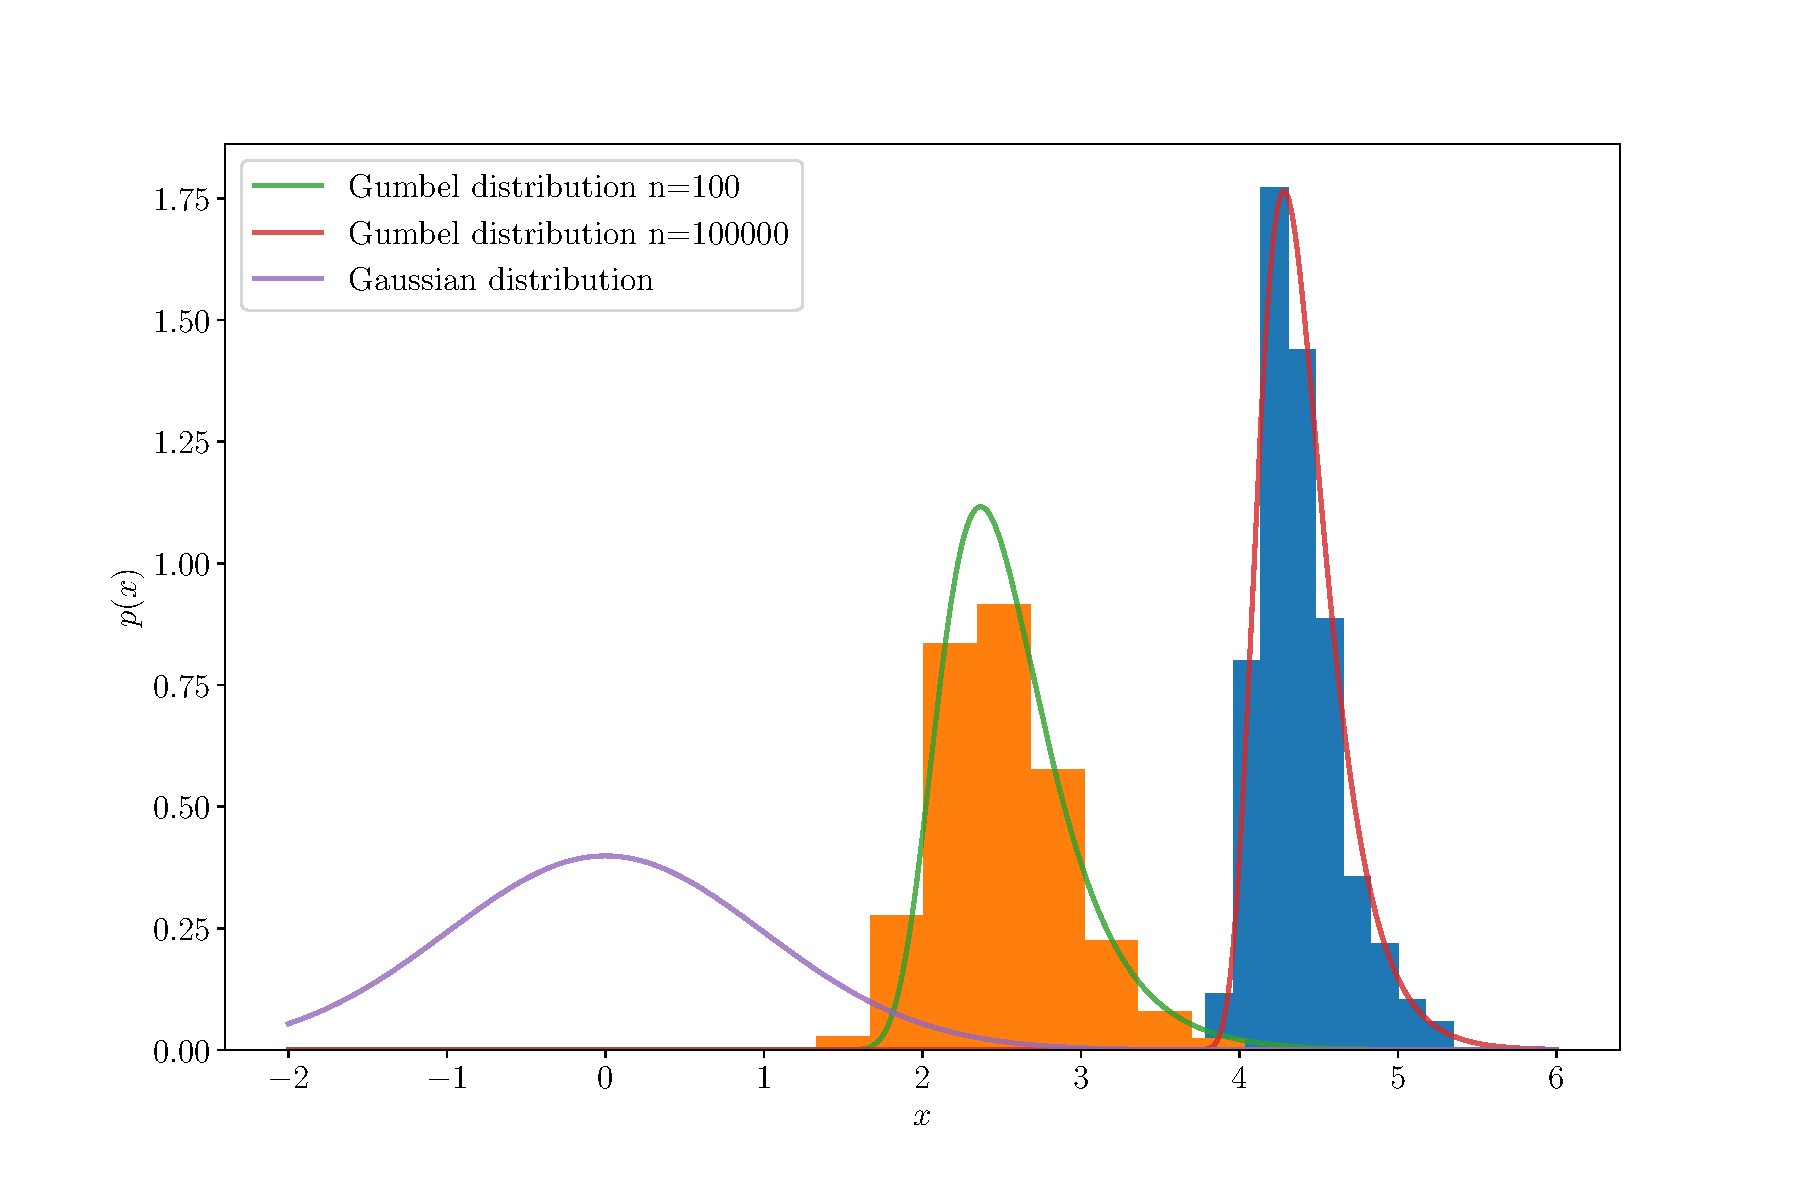
\includegraphics[width=0.8\linewidth]{figures/gumbel_uni.pdf}
    \caption{Gumbel distribution}%
    \label{fig:gumbel_uni}
\end{figure}

Since the latent space is approximately standard normally distributed one way
to approach sampling from outliers is extreme value theory. Extreme value
theory is the theory of the distribution of maxima of sequences of independet,
identically distributed random variables. Let $z_1, \dots, z_n$ be a sequence
of i.i.d. standard normally distributed random variables, then the asymtotic
distribution of the maxima $M_n = \max (z_1, \dots, z_n)$ is
\begin{equation}%
    \label{eq:gumbel_distribution}
    P{a_n ( M_n - b_n ) < x} \rightarrow e^{-e^{-x}}
\end{equation}
where
\begin{equation}
    \begin{aligned}%
        \label{eq:gumbel_params}
        &a_n = (2 \log n )^{1/2} \\
        &b_n = (2 \log n )^{1/2} - \frac{1}{2} (2 \log n )^{1/2} (\log \log
        n + \log 4 \pi)
    \end{aligned}
\end{equation}
\citep{leadbetterAsymptoticDistributionsExtremes1983}.

As an example, \autoref{fig:gumbel_uni} shows the distribution of the maxima of
sequences of length $n = 100$ and $n = 100000$ drawn i.i.d. from a standard
normal distribution in comparison.
\begin{figure}[htpb]
    \centering

    \begin{subfigure}[]{0.48\textwidth}
        \centering
    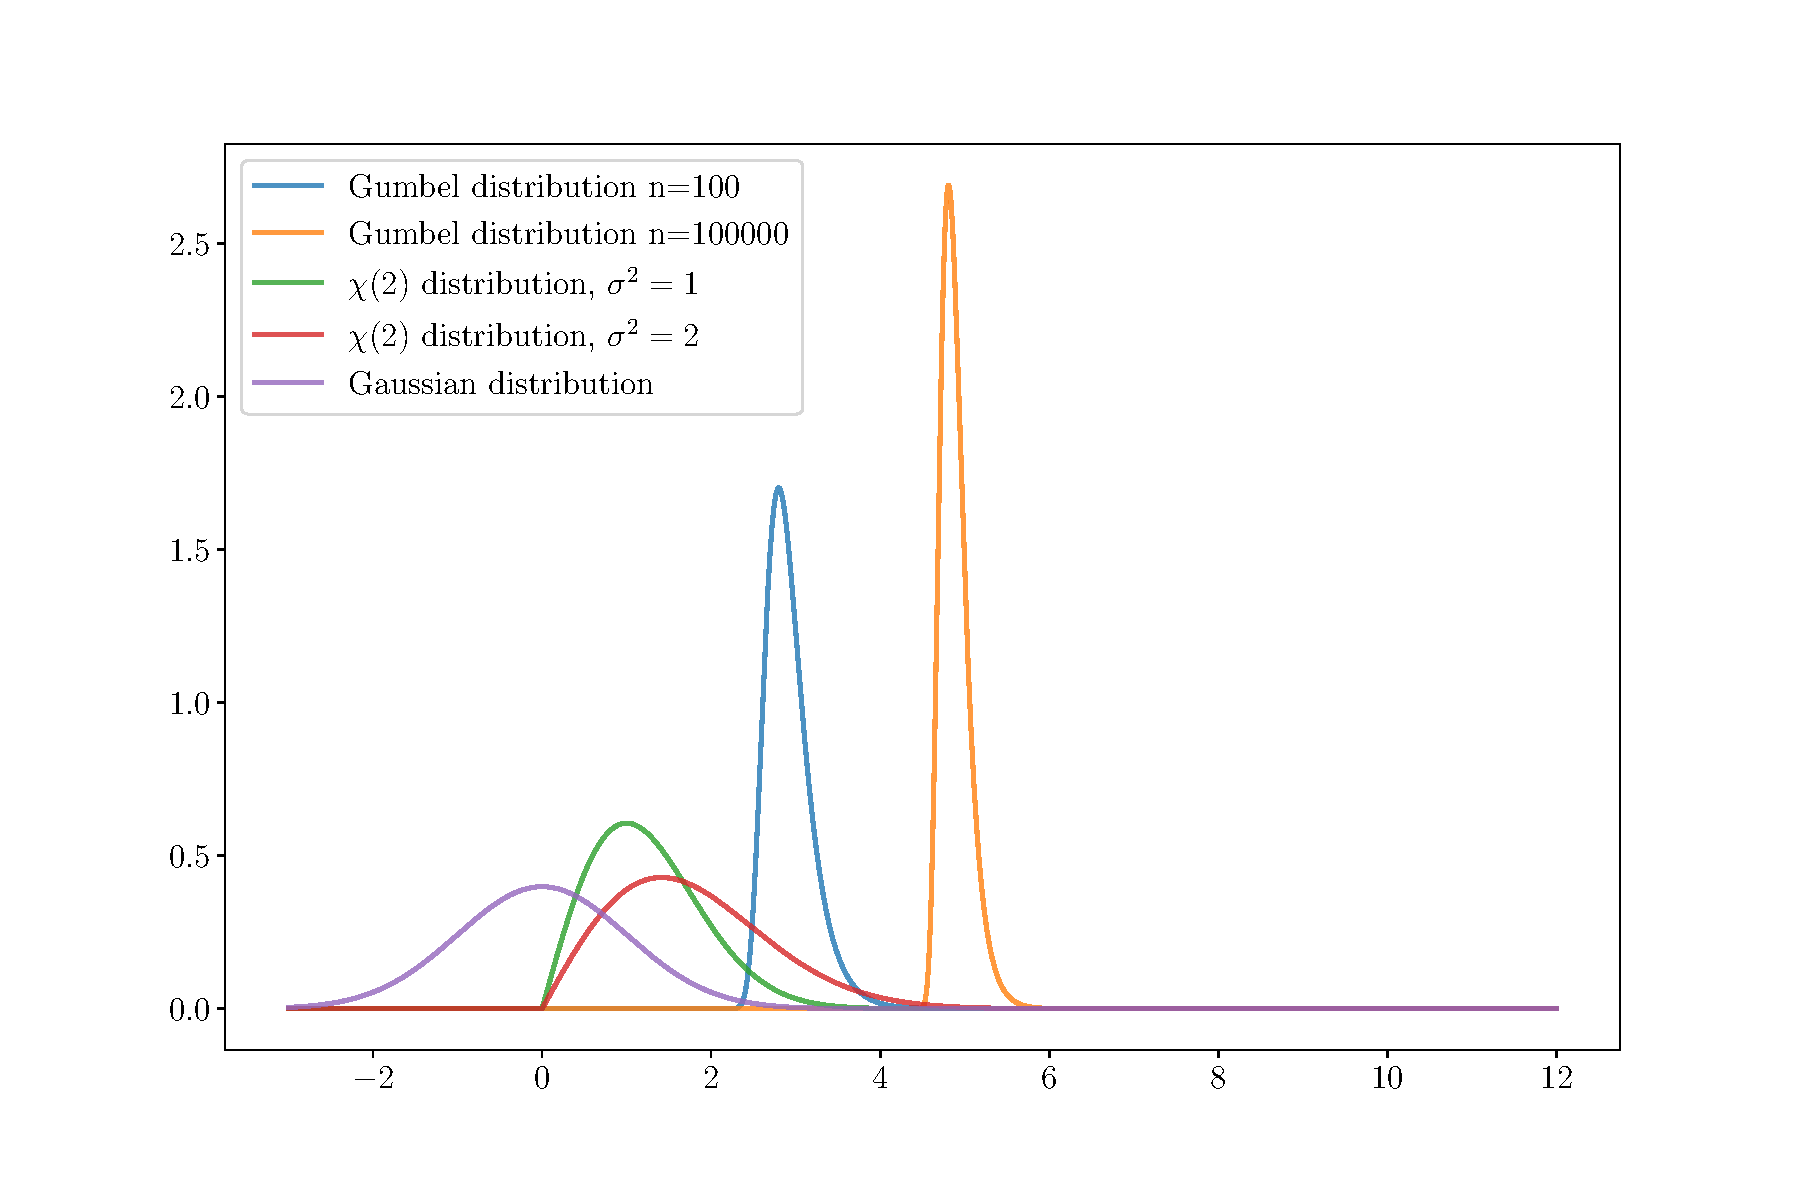
\includegraphics[width=\linewidth]{figures/gumbel_multi_2.pdf}
    \caption{}
    \label{fig:}
    \end{subfigure}
    \begin{subfigure}[]{0.48\textwidth}
        \centering
    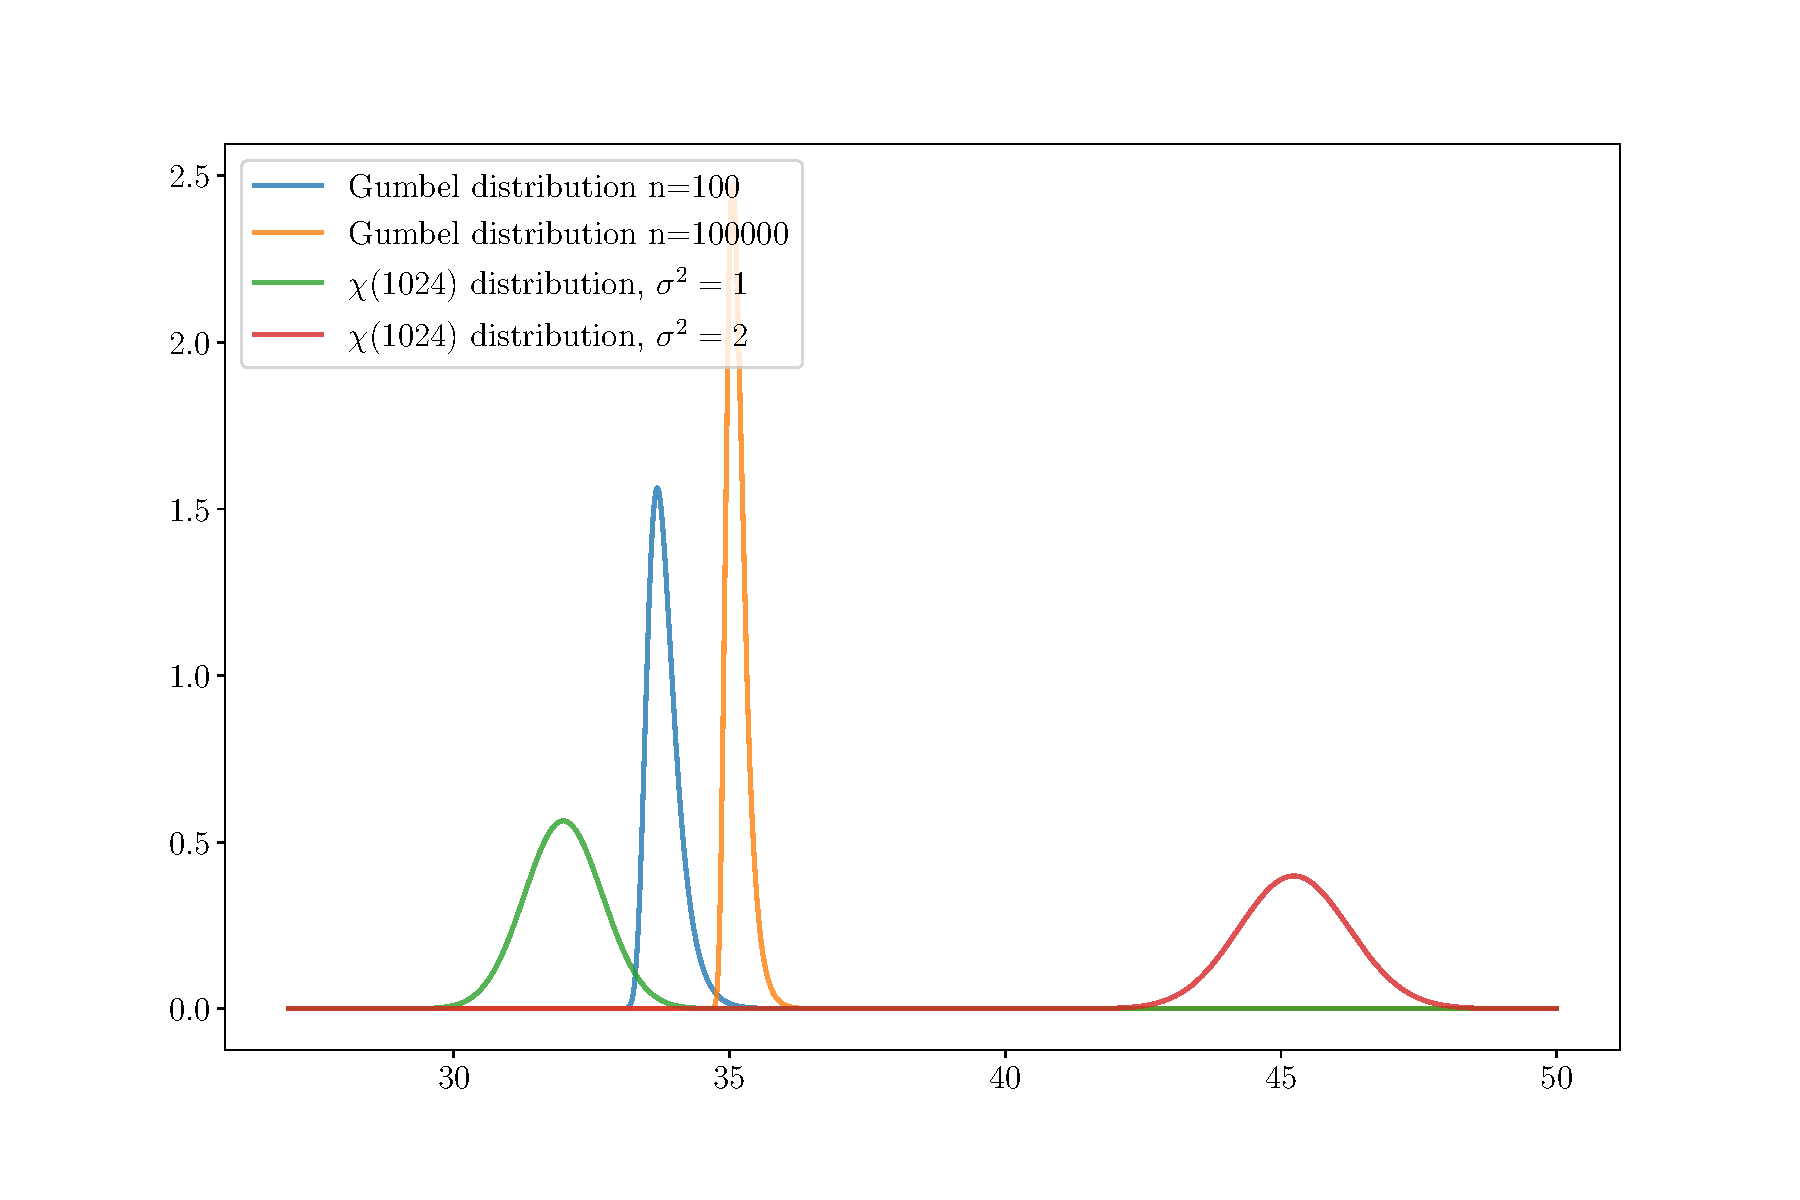
\includegraphics[width=\linewidth]{figures/gumbel_multi_1024.pdf}
    \caption{}
    \label{fig:}
    \end{subfigure}

    \caption{Gumbel distribution}%
    \label{fig:gumbel_multi}
\end{figure}

This method of sampling outliers is especially useful in lower dimensions, as
we cannot use the methods established in
\autoref{sub:high_dimensional_gaussian_distributions}. We can see in
\autoref{fig:gumbel_multi}, that for $d=2$ the distribution of the lengths of
the random vectors is still rather close to a standard normal distribution, and
indeed doubeling the variance does not lead to a distribution that is noticably
different from the data distribution. For $d=1024$, as is the case for the
image data used for the experiments, we can use the previously introduced
method of sampling from a latent distribution with higher variance, as this
leads to a significantly distinct distribution.

\section{Geometrical Approach}%
\label{sec:geometrical_approach}

% Do we even need this?
% Dirichlet Distribution
% Sampling from the edge/outside of the simplex
% Splitting of latent space

% TODO: Citing
In order to make use of the archetype representation of our data we need to
sample archetype coefficients. Sampling from our deep archetypal architecture
can be done as follows. The archetypes, wether they are updated during training
or not, are taken to be fixed and saved. For a fixed configuration of
archetypes the coefficients $a_{ij}$ can be sampled from a Dirichlet distribution,
a generalization of the beta distribution for the multivariate case. For $k$
archetypes and shape parameters $c_i > 0, i = 1, \dots, k$ the probability
density function of the Dirichlet distribution is
\begin{equation}%
    \label{eq:dirichlet_pdf}
    p(a_i) = \frac{ \Gamma ( \sum_j c_j ) }{ \prod_j \Gamma (c_j) } \prod_j
    a_{ij}^{c_j - 1}
\end{equation}
\citep{forbesDirichletDistribution2010}

Since the archetypes are already extreme examples we can control how atypical
the samples should be and furthermore what features we want to be extreme by
controlling the shape parameters.

Once $N$ samples have been drawn we can compute samples from the
$(k-1)$-dimensional latent space.
\begin{equation}%
    \label{eq:aa_k_sample}
    \mathbf{t}_i' = \sum_j a_{ij} \mathbf{z_{j,\mathrm{fixed}}}
\end{equation}

In additon to the layers that map data from the latent space of the invertible
neural network to the archetype space we need to train a layer that
approximates the inverse to this, as a mapping to the $(k-1)$-dimensional
subspace is in general not invertible. Details on how this layer is trained can
be found in \autoref{sec:network_architecture}
\begin{equation}%
    \label{eq:aa_upsample}
    \mathbf{t}_i = f_C (\mathbf{t}_i')
\end{equation}
Finally we can use the neural network to get samples in data space
\begin{equation}%
    \label{eq:aa_to_data}
    \mathbf{x}_i = \mathrm{INN}^{-1} (\mathbf{t}_i)
\end{equation}

Additional modifications can be applied: We can add gaussian noise to the
samples in any of the latent spaces to get more variation or more extreme
samples.

Another modification is to add a random sample to $\mathbf{t}_i$ from the
nullspace of the mapping to the archetype space to mitigate the loss of
information that occures.
% TODO: Finish nullspace

\section{Discriminator Training}%
\label{sec:discriminator_training}

% Combined loss function
% Compare with og paper

\section{Network Architecture}%
\label{sec:network_architecture}

% Architecture of the INN
% Adding the AA layers

\section{Datasets}%
\label{sec:datasets}

% EMNIST
% Also discuss the specifics of the datasets in EMNIST
% FERG

